

\chapter{Wprowadzenie do algorytmów heurystycznych}
\section{Algorytmy heurystyczne i metaheurystyczne}
 Optymalizacja rozwiązań wykorzystywana jest w prawie każdym aspekcie życia. Podwyższanie jakości usług, obniżanie kosztów wyrobów, czy minimalizacja zużycia surowców to bardzo popularne zagadnienia optymalizacyjne. Medycyna, logistyka, ekonomia to przykłady dziedzin, w których optymalizacja znajduje swoje zastosowanie. 
 Optymalizacja to minimalizacja bądź maksymalizacja pewnej funkcji, zwanej często funkcją oceny, która określa jakość rozwiązania danego problemu. Znalezienie minimum lub maksimum wymaga więc wyznaczenia funkcji oceny dla każdego możliwego rozwiązania problemu i wyborze rozwiązania o najlepszej wartości funkcji oceny. Niestety często rozmiar zadania, dla którego szukamy optymalnego rozwiązania, jest tak duży, że sprawdzenie wszystkich rozwiązań, bądź zastosowanie algorytmu znajdującego najlepsze rozwiązanie nie jest możliwe ze względu na zbyt długi czas wykonania. Liczba operacji, które należy wykonać często rośnie wykładniczo wraz ze wzrostem rozmiaru problemu. Stwarza to możliwość zastosowania heurystyk.
 
 ,,Terminem heurystyka (z języka greckiego heurisko - znajduję) określa się sposób postępowania oparty na zdobytym doświadczeniu, wykorzystaniu istniejących faktów i reguł, w celu znalezienia odpowiedzi na postawione pytanie"\cite{Algorytmy:Widuch}. Algorytmy heurystyczne to takie algorytmy, które na podstawie przebiegu obliczeń i otrzymywanych wynikach, starają się znaleźć jak najlepsze rozwiązanie problemu, jednak zwykle nie jest to rozwiązanie optymalne (tj. najlepsze wśród wszystkich możliwych rozwiązań). W zamian za możliwość otrzymania nieco gorszego rozwiązania uzyskamy krótszy czas działania algorytmu. Algorytmy heurystyczne wykorzystywane są w przypadku, gdy dokładne algorytmy są z przyczyn technicznych zbyt kosztowne, lub gdy są nieznane (np. dla problemu przewidywania pogody). Często też używa się heurystyk by ,,nakierować'' gotowy algorytm na rozwiązanie optymalne, co w rezultacie skróci czas jego wykonania.
 
 Algorytmy heurystyczne możemy podzielić ze względu na sposób, w jaki generowane są nowe rozwiązania:
 \begin{itemize}
 	\item Algorytmy probabilistyczne - wykorzystują czynnik losowości; często kolejne rozwiązanie wybierane jest losowo z określonej puli rozwiązań. Może to doprowadzić do różnych wyników końcowych otrzymanych w kolejnych wykonaniach algorytmu.
 	\item Algorytmy deterministyczne - nie zawierają czynnika losowego. Otrzymywane rozwiązanie jest zawsze takie same, przy każdym wykonaniu algorytmu na takich samych danych wejściowych. 	
 \end{itemize}

W niektórych algorytmach wykorzystane są dwie heurystyki, nadrzędna i podrzędna. Pierwsza z nich steruje i uzupełnia działanie drugiej heurystyki. Takie podejście nazywane jest przez niektórych badaczy metaheurystykami \cite{Algorytmy:Widuch}. Inna definicja metaheurystyki to ,,procesy iteracje działające zgodnie z klasyczną metodą heurystyczną, wspomagane inteligentnie przez różne koncepcje eksplorowania i eksploatowania przestrzeni rozwiązań z użyciem technik uczących. Wspomaganie to ustrukturalnia informacje w celu sprawnego znalezienia rozwiązań bliskich optymalnemu" \cite{Metaheurystyki:Osman}. Po raz pierwszy termin metaheurystyki został użyty przez Freda Glovera w 1986 roku jako określenie algorytmów, które nie rozwiązują bezpośrednio żadnego problemu, lecz określają w jaki sposób budować algorytmy podrzędne w celu uzyskania rozwiązania \cite{Future:Glover}.

\section{Algorytm wyszukiwania z tabu}

Przykładem algorytmu metaheurystycznego jest algorytm wyszukiwania z tabu (ang. \textit{Tabu Search}). Algorytm ten został zaproponowany w 1977 r. kiedy to Fred Glover przedstawił pracę na temat wykorzystania pamięci krótkotrwałej i długotrwałej w przeszukiwaniu lokalnym. Pamięć krótkotrwała służyła do zapamiętywania ostatnich ,,ruchów'' algorytmu i była modyfikowana przez kolejne jego iteracje (pamiętane były wybrane wartości wykorzystywane przez algorytm w ostatnich iteracjach). Natomiast pamięć długotrwała miała na celu pamiętanie najbardziej atrakcyjnych rozwiązań przestrzeni poszukiwań. To właśnie w oparciu o tą zasadę, Glover zaproponował w 1986 r. algorytm \textit{Tabu Search}. Glover jest uznawany za autora algorytmu mimo tego, że w tym samym roku Michael Hansen opublikował pracę opisującą bardzo podobną heurystykę. Na przestrzeni lat algorytm został ulepszony i aktualnie dostępnych jest wiele jego różnych wersji, np. \textit{Probabilistic Tabu Search} lub \textit{Reactive Tabu Search}.

\subsection{Zasada działania algorytmu}

Wyszukiwanie z tabu to metaheurystyka służąca do rozwiązywania problemów optymalizacji. Algorytm oparty na tej metaheurystyce dokonuje iteracyjnego przeszukiwania przestrzeni rozwiązań, z użyciem tzw. sąsiedztwa oraz na zapamiętuje ostatnio wykonane ruchy w celu uniknięcia ich powtarzania. Wywodzi się on bezpośrednio z metody przeszukiwania lokalnego, jednak jest od niej zdecydowanie skuteczniejszy dzięki możliwości ,,wychodzenia'' z minimów lokalnych. Podstawą tej możliwości jest zaakceptowanie gorszego aktualnego rozwiązania w celu uzyskania rozwiązania lepszego. Możliwe jest to dzięki uaktualnianiu danych tabu, czyli listy ruchów, które algorytm już wykonał, co zabezpiecza algorytm przed powrotem w obszary przestrzeni rozwiązań już przeszukane. Obecność ruchów na liście tabu jest tymczasowa, co w konsekwencji blokuje dany ruch przez określoną liczbę iteracji (rysunek 2.1). Możliwe jest złamanie tej zasady, ale tylko wtedy, gdy ruch spełnia tzw. kryterium aspiracji. Warunkiem zakończenia działania algorytmu jest najczęściej wykonanie określonej liczba iteracji lub osiągnięcie satysfakcjonującego rozwiązania. Możliwe jest również monitorowanie aktualnego wyniku i, jeżeli nie ulega on poprawie przez określoną liczbę iteracji, zatrzymanie wykonania algorytmu. Pseudokod działania algorytmu przedstawiony został na rysunku 2.2.

\begin{figure}
	\centering
	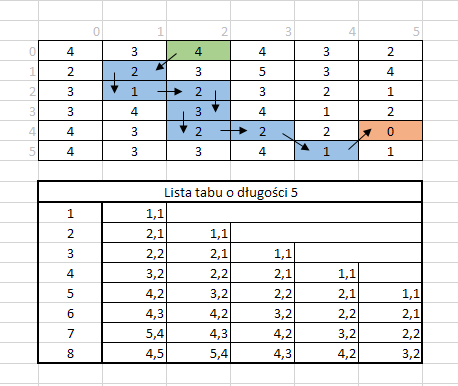
\includegraphics{TabuSearchIL}
	\caption{Proces wyszukiwania z tabu}
	\label{fig: TabuSearchIL}
\end{figure}

\begin{figure}
	\centering
	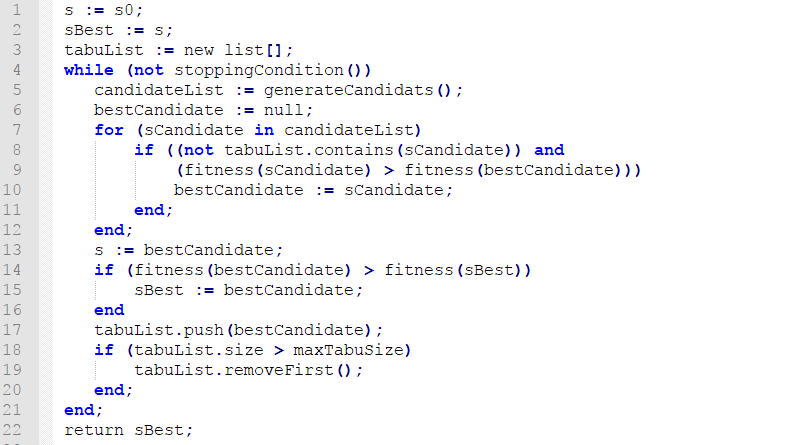
\includegraphics{PseudokodTabu}
	\caption{Pseudokod algorytmu wyszukiwania z tabu}
	\label{fig: AlgorytmTabu}
\end{figure}

\subsection{Sąsiedztwo rozwiązania}

Najważniejszym czynnikiem, od którego zależy sukces algorytmu jest poprawnie zdefiniowane sąsiedztwo, które będzie przeszukiwane w danej iteracji. Do sąsiedztwa powinny należeć rozwiązania różniące się w sposób nieznaczny od rozwiązania bieżącego. Jednak sąsiedztwo powinno umożliwiać algorytmowi przejście w każdy obszar przestrzeni rozwiązań. Sposób w jaki definiowane jest sąsiedztwo zależy od danego problemu i typu jego rozwiązań. Rozwiązania problemu mogą być reprezentowane np. przez wektory binarne, wektory liczb rzeczywistych, czy dowolne permutacje elementów zadanych zbiorów. Jeżeli na przykład rozwiązaniem będzie permutacja pewnego zbioru \textit{n} elementowego, to sąsiedztwem możemy określić jedno z trzech typów przejść (ruchów) między permutacjami:

\begin{itemize}
	\item wstaw(x, y) - wstawienie elementu y na pozycję x (permutacje z powtórzeniami),
	\item zamień(x, y) - zamiana elementów na pozycjach x i y,
	\item odwróć(x, y) - odwrócenie kolejności występowania elementów, począwszy od elementu o indeksie x, aż do elementu na pozycji y.
\end{itemize}

Sąsiedztwem danej permutacji będzie więc każda inna permutacja uzyskana za pomocą, wybranego na początku, sposobu modyfikacji bieżącej permutacji. Dzięki tak zdefiniowanemu sąsiedztwu możliwe jest łatwe zidentyfikowanie ruchu za pomocą pary indeksów (x, y). Para ta zostanie zapisana na liście tabu, a ruch ten będzie zablokowany przez następne iteracje.

Może się jednak okazać, że generowane sąsiedztwa są zbyt duże, by każdorazowo przeszukiwać je w całości. Stosowane jest wtedy zawężanie sąsiedztwa. Jednym ze sposobów zawężania jest losowy dobór sąsiedztwa. Wprowadza to element probabilistyczny do algorytmu, co zmniejsza prawdopodobieństwo powstania niepożądanych cykli. Jednak przy takim podejściu możemy pominąć obszary przestrzeni rozwiązań, w których znajduje się rozwiązanie optymalne.

\subsection{Kryteria aspiracji}

Może się zdarzyć, że zablokowanie pewnych ruchów doprowadzi do stagnacji procesu przeszukiwania lub całkowicie zablokuje kolejny ruch (np. w sytuacji, gdy wszystkie możliwe ruchy są na liście tabu). Jest to możliwe, ponieważ algorytm przechowuje tylko atrybuty rozwiązań, a nie całe rozwiązania. Kryterium aspiracji umożliwia zapobieganiu takiej sytuacji.
Spełnienie kryterium aspiracji pozwala na złamanie zakazu tabu, czyli wykonanie ruchu, który znajduje się na liście ostatnio wykonanych. Najpopularniejszym i najprostszym kryterium aspiracji jest uzyskanie najlepszego, nieznanego jak dotąd, wyniku. Musi być ono lepsze od aktualnie najlepszego w celu uniknięcia zapętleń. Jednak większość kryteriów aspiracji jest bardziej skomplikowana i opiera się na wyspecjalizowanym przewidywaniu możliwości powstania cyklu po wykonaniu określonego ruchu.

\subsection{Dywersyfikacji i intensyfikacja obszaru poszukiwań}

Ważnym aspektem algorytmu wyszukiwania z tabu jest pamięć długoterminowa. Służy ona do przechowywania danych o wykonanych już iteracjach i do budowania statystyk. Dzięki tym statystykom można modyfikować strategię poszukiwania. Głównym celem takich modyfikacji może być spełnienie jednego z dwóch kryteriów:
\begin{itemize}
	\item Intensyfikacja - jeżeli według statystyki, w danym obszarze znajduje się dużo dobrych rozwiązań to algorytm zagęści obszar poszukiwań. Dzięki temu istnieje szansa na znalezienie jeszcze lepszego rozwiązania w danym obszarze.
	\item Dywersyfikacja - jest to powiększenie obszaru poszukiwań. Najczęściej stosowanym sposobem jest nakładanie kary na ruchy, które powtarzają się w perspektywie dłuższego czasu. Efektem tego jest ,,przeniesienie" algorytmu w inne rejony poszukiwań, co zmniejsza szanse na pominięcie najlepszych rozwiązań.
\end{itemize}
Wykorzystanie intensyfikacji i dywersyfikacji w znaczniej mierze poprawia efektywność algorytmu, dlatego kryteria te są wykorzystywane w większości nowych wersji algorytmu \textit{Tabu Search}.




